\chapter{Introduction}
\label{sec:Introduction}
% Thesis statement. 

%Particle colliders allow us to study quantum chromodynamics (QCD), 

% Study nuclear physics
One of the major goals of high-energy physics is to study quantum chromodynamics (QCD), the theory of the strong nuclear force which describes the interactions between quarks and gluons.
Quarks and gluons are the building blocks of atomic matter; every proton has two up quarks and a down quark, and every neutron has two down quarks and an up quark. 
Gluons mediate the interactions between those quarks.
Despite their prominance, these particles are never observed in isolation under standard terristrial conditions.
They are always found together in the form of hadrons, which are particles such as protons and pions that have two or three quarks bound together.
This phenomenon, the fact the quarks are not normally observed in isolation, is called confinement.
However, at sufficiently high density and temperature, it is possible to have a medium that is too hot for hadrons.
Instead, the quarks and gluons exist freely, and their collective behavior exhibits fluidlike properties \cite{Heinz:2005zg}.
This medium is called the quark-gluon plasma (QGP).
By studying the QGP, as well as the conditions that exist after the QGP dissipates, physicists can get more insight into the strong nuclear force.

Modern particle accelerators create conditions under which the QGP can exist for a short time \cite{Heinz:2000bk}.
This is primarily done via the collision of heavy ions such as $\ce{^197 \mathrm{Au}}$ and $\ce{^208 \mathrm{Pb}}$.
At energies seen by the Large Hadron Collider (LHC), where the ions have center of mass energies per nucleon on the order of tera electron Volts (TeV), these collisions can produce a hot, dense medium from which thousands of particles are emitted \cite{Aamodt:2010cz}.
This medium (the QGP and subsequent hadronic phase) has several names, such as "interaction region" or "particle-emitting source", though it is colloquially called a fireball.
The collision, the medium, and the subsequently emitted and measured particles are collectively known as an event. 

\section{Heavy-ion collisions}
\label{sec:HeavyIonCollisions}

\begin{figure}[hbt]
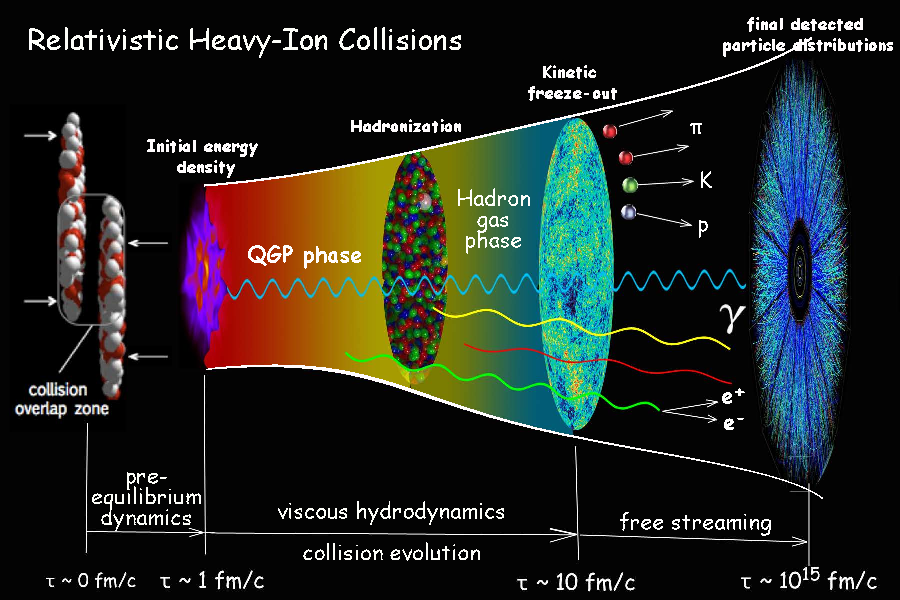
\includegraphics[width=36pc]{Figures/BorrowedFigures/HeavyIonEvolution.pdf}
\caption[Evolution of a heavy ion collision]{Evolution of a heavy ion collision \cite{Shen:2015msa}. 
Two ions collide and leave behind a medium of high energy density. 
After about 1 fm/$c$, the medium thermalizes as a plasma of deconfined quarks and gluons. 
After a few fm/$c$, the quarks and gluons cool down and hadronize into pions, kaons, and many other particles. These hadrons scatter off each other few more fm/$c$, until the become so dilute that they free-stream to a detector.}
\label{fig:HeavyIonEvolution}
\end{figure}


Figure \ref{fig:HeavyIonEvolution} shows a cartoon of a heavy ion collision.
It is suspected that the QGP exists for only a few moments after the collision of these ions, on time scales of about a few fm/$c$ (1 fm/$c$ = $10^{-15} \mathrm{m}/c \sim 10^{-23}$ seconds).
Over time the plasma expands and cools, and eventually the quarks and gluons combine to form hadrons, a process called hadronization.
In the subsequent hadronic phase, the hadrons scatter off each other in an elaborate billiard ball game, with particles near the edge of the expanding fireball having the possibility to free-stream to the detector.
Eventually, the source becomes dilute enough that the inter-particle scatterings die off. This occurs on time scales on the order of 10 fm/$c$ \cite{BraunMunzinger:2007zz}.
While people often speak of a singular kinetic freezeout time (the time when the rescatterings cease), in actuality particles are emitted at varying rates throughout the lifetime of the fireball.

Heavy-ion physics programs such as ALICE (A Large Ion Collider Experiment) seek to study the evolution of these fireballs.
The field tries to answer questions such as "When does hadronization occur?", "What equations of state describe the evolution of the interaction region?", "What interactions are occuring between particles during during this evolution?", and "What is the size and shape of the source at kinetic freezeout?".
A number of models have been developed to probe these questions and others \cite{Werner:2010aa,Karpenko:2012yf,Bozek:2012qs,Schenke:2009gb}, and experimental data help refine these models.

Loosely speaking, a collision model has three main components: initial conditions describing the shape and energy density of the source; a theory describing how the system evolves over time; and the final result of collision, namely a description of the particles that are emitted including their momenta, emission time, etc.
%Collider experiments have been designed so as to simplify assumptions about the initial conditions of fireballs.
Collider experiments have been designed to simplify assumptions about the initial conditions of fireballs, and to measure their asymptotic state.
$\ce{^197 \mathrm{Au}}$ and $\ce{^208 \mathrm{Pb}}$ ions are used since these particles have a spherical symmetry to their nuclear structure that gives the fireballs a relatively simple initial geometry.
Particle collider experiments provide insight into the final state of collisions by measuring the final momenta of particles produced in millions of events.

% Heavy-ion models act as a bridge...
%In the last 15 years, the Relativistic Heavy Ion Collider (RHIC) has performed Au--Au and U--U collisions, and the Large Hadron Collider (LHC) has done Pb-Pb collisions.

%By looking at the final-state information of large ensembles of collisions and making various model assumptions about the initial conditions and evolution, it is possible to work backward to obtain a better grasp of what happens in the early stages of the collisions.
%To answer many of the above questions, it is often necessary to look at this final-state information and work backwards.


Beyond simply measuring asymptotic particle momenta, collider experiments can use an assortment of analysis techniques to probe various facets of the fireball evolution.
These techniques include flow analysis \cite{Aamodt:2010pa,Heinz:2013th}, the study of particle spectra \cite{Aamodt:2010cz}, and an interferometry technique known as femtoscopy \cite{Aamodt:2011mr,Lisa:2005dd}.
In the following sections, we'll give a brief introduction to these topics, before moving on to the main topic of this thesis: femtoscopy.



%In this thesis, we will focus our discussion on the ways that femtoscopy is capable of shedding light on both the spatial characteristics of the particle-emitting source, as well as the interactions between particles created within the source.
% In particular, we will focus on the new avenues of research available with baryon femtoscopy, and ... lambda baryon ($\Lambda$).
\subsection{Jet quenching}


\subsection{Flow}
\label{sec:Flow}

Figure \ref{fig:Almond} shows a cartoon of a peripheral heavy-ion collision.


\begin{figure}[hbt]
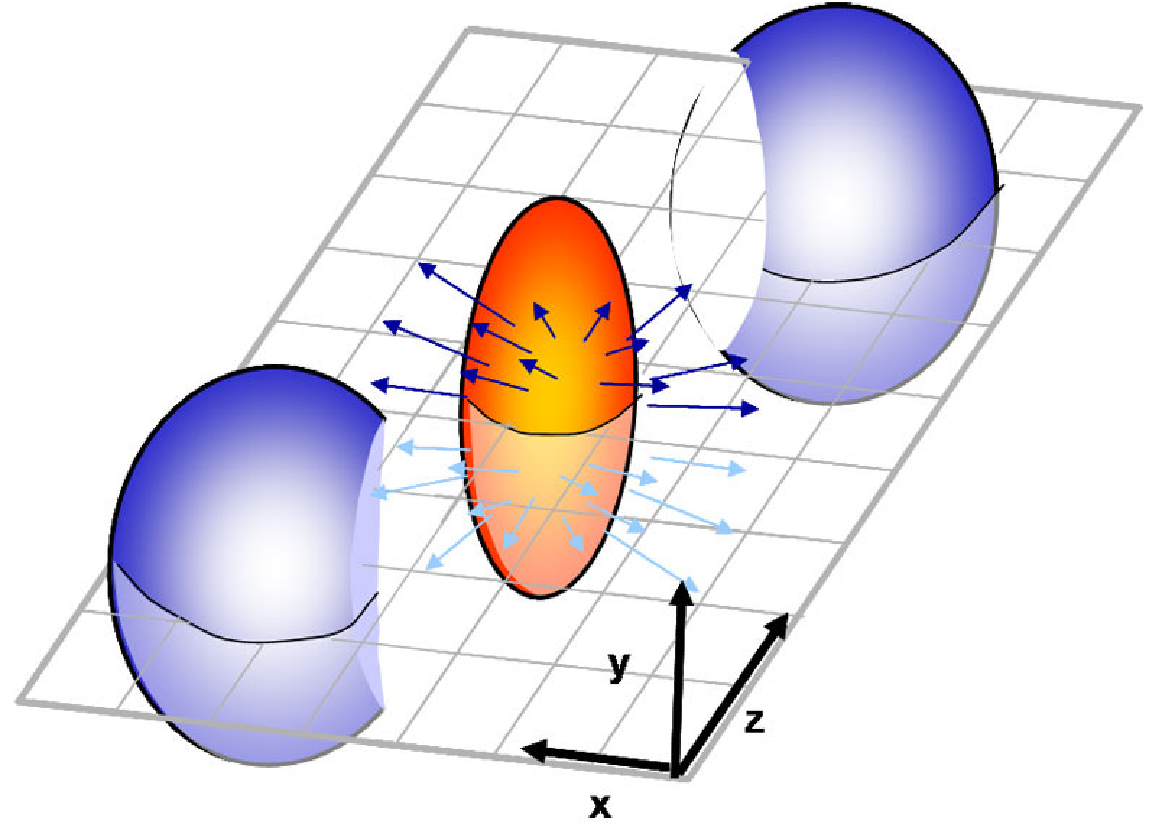
\includegraphics[width=36pc]{Figures/BorrowedFigures/Almond.pdf}
\caption[Non-central collision]{ 
Cartoon of a non-central heavy-ion collision \cite{Rapp:2008qc}.
The blue shapes are the recently-collided ions, while the overlap region of the expanding fireball is orange.
The almond-shaped fireball is taller than it is wide, which results in a larger pressure gradient along the x-axis than along the y-axis.
This pressure gradient causes the fireball to expand more rapidly along the x-axis than along the y-axis.

}
\label{fig:Almond}
\end{figure}


\subsection{Spectra}

If the fireball of a heavy-ion collision is in an evolving thermal equilibrium as hydrodynamic models suggest, what is the temperature of the fireball at different points in its lifetime? 
Answers to this question can be found by looking at particle spectra.
Spectral analyses measure the number of particles produced in collisions.
There are a few ways to disect this information.
For each species of particle (e.g.\ $\pi$, K, p), one can look at how many of them are produced on average for a given event.
For a system in thermal equilibrium, the expected number of particles $n_i$ of a particular species in a given energy state $E_i$ follows the distribution
\begin{equation}
\label{eq:ThermalDistribution}
n_i(E_i) = \frac{g_i}{e^{(E_i - \mu_b)/kT} \pm 1}
\end{equation}
where $g_i$ is the degeneracy of the state, $\mu_b$ is the baryochemical potential of the system,  $T$ is the temperature of the system, and the  $+/-$ is for fermions/bosons. 
The baryochemical potential quantifies the baryon-antibaryon asymmetry of the system; $\mu_b = 0$ means that there are equal numbers of baryons and antibaryons.
% citation needed

%One can also look at the momentum distribution of a particular particle species

\begin{figure}[hbt]
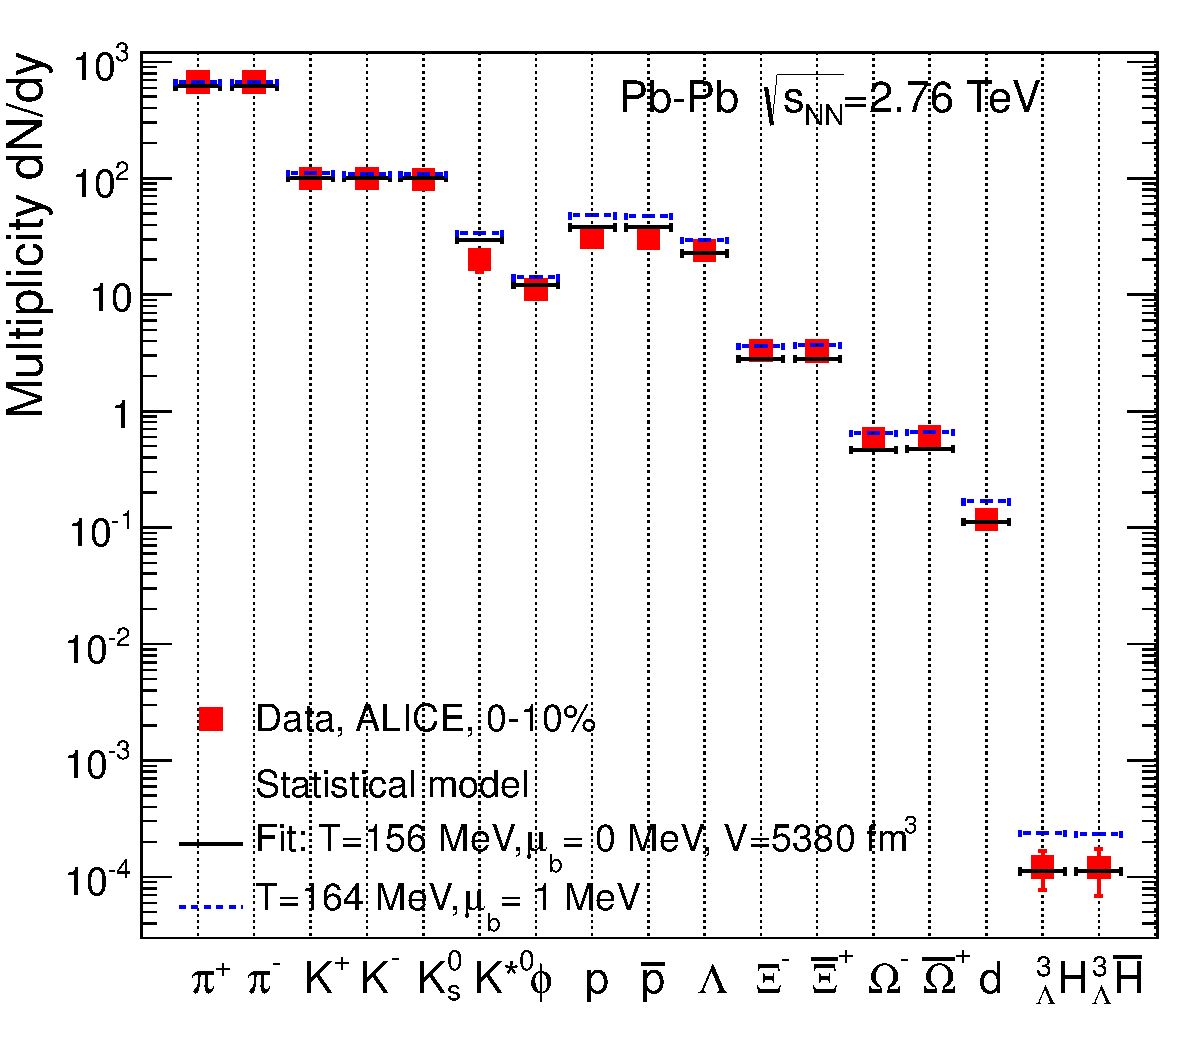
\includegraphics[width=36pc]{Figures/BorrowedFigures/ALICEYieldsThermalFit.pdf}
\caption[Thermal fit of ALICE yields]{Particle yields from central Pb-Pb collisions at ALICE, which are fit with a statistical hadronization model \cite{Stachel:2013zma}. 
The fit suggests that the particle abundances, which mostly appear to obey a thermal distribution, cease to evolve below the temperature $T = 156$ MeV .
The fit also finds that the baryon chemical potential is zero, which means that there is no asymmetry between the matter and antimatter yields of the system. 
}
\label{fig:ThermalYieldFit}
\end{figure}

Figure \ref{fig:ThermalYieldFit} shows particle yields measured in central Pb-Pb collisions at ALICE.
Those yields have been fit with a thermal model \cite{Stachel:2013zma}. 
The fit finds that the baryochemical potential is zero, as one expects at LHC energies.
Most of the particle species appear to obey a thermal distribution for $T = 156$ MeV, which suggests that relative particle yields cease to evolve below that temperature.
That said, the proton and antiproton yields both lie a couple sigma below the thermal value, and studies are ongoing to determine what physics effects might drive these particles out of equilibrium.


\section{Femtoscopy (HBT)}
\label{sec:FemtoHBT}
Hanbury-Brown and Twiss first used two-particle interferometry of photons to measure the angular size of the star Sirius \cite{HanburyBrown:1956bqd}.
Later, it was observed that similar techniques could be employed in a laboratory setting with pions ($\pi$) to characterize the size of particle collisions \cite{Goldhaber:1960sf}.
This process of measuring two-particle correlations for pairs of particles with very similar momentum is often referred to as HBT, after the progenitors of the technique.
HBT was originally used to study photons and later used to look at pions, so it often carries a connotation of Bose-Einstein correlation effects, i.e. the quantum mechanical tendency of identical bosons to exist in the same state. This is in contrast to Fermi-Dirac statistics, wherein identical fermions cannot occupy the same state because of the Pauli exclusion principle.
Modern analyses look at all manner of hadrons, and therefore the correlations might be subject to bosonic, fermionic, or non-identical particle statistics.
In the nuclear physics context, the focus of these analyses is on measuring very small sources, so the more general term \textit{femtoscopy} has come into use.

As will be discussed in Section \ref{sec:CorrelationFunctionModel}, there is a correlation between the relative position of the particles at their moment of last scattering and their subsequent momentum at freezeout.
The relative position of the particles can be described by a two-particle emission function. The final state of the particles, including their momenta, depends on the interactions between the particles and is accounted for by the two-particle wave function of the pair.

Femtoscopic analyses are capable of probing both the two-particle emission function (i.e the size and shape of the source) and the interactions between particles. 

The primary tool of femtoscopy is the correlation function.
A femtoscopic correlation function is constructed by binning the momentum difference (usually called relative momentum) of pairs of particles.
This is done for both a signal distribution and a background distribution, and the correlation function is the ratio of the two.
Correlation functions are normalized such that a value of unity for a given bin suggests that there are no correlated effects between the particles in that bin.
A value above unity means that some effect is causing an increase of pairs at a given relative momentum, while a value below unity (but never below zero) suggests that some effect is supressing pairs at that relative momentum.
More details on the experimental construction of correlation functions can be found in Section \ref{sec:CorrelationFunctionConstruction}.

% chaotic source
\section{Femtoscopic sources}
\label{sec:FemtoSources}


%In the context of both astronomy and particle physics, HBT/
Femtoscopy is built on measuring the interference patterns of particles emitted incoherently from a source.
Femtoscopic analyses are capable of measuring both spatial and temporal characteristics of these sources.


As will be discussed in greater detail in Section \ref{sec:CorrelationFunctionModel}, femtoscopy does not actually measure the size of the full interaction region at the time of freezeout.
Rather, it measures the size of the region in which particles are emitted with the same momentum, also called the region of homogeneity \cite{Akkelin:1995gh}.
If particles were emitted isotropically throughout the interaction region, the measured source size would be the the full size of the interaction region.
However, effects such as radial flow create correlations between particle emission direction and position. 
For example, a particle near the edge of the fireball is more likely to be emitted outward, where there are fewer particles to scatter off of, than it is for it to be emitted inward where it would have to travel through the bulk of the interaction region without scattering again. 
The homogeneity radii measured by femtoscopy give a snapshot of the final conditions of the fireball.
These final conditions can help theorists tune their evolution models.

Femtoscopic analyses traditionally study pions \cite{Goldhaber:1960sf,Aamodt:2011mr} because of their ready availability.  
However, measurements of heavier particles such as kaons \cite{Abelev:2012ms} and baryons \cite{Gos:2007cj} can serve to complement the pion results.  
One motivation for studying an assortment of heavier particles is to test the hydrodynamic prediction that radial flow should cause the source radii to scale roughly as the inverse of the transverse mass $1/m_{\mathrm{T}} = (m^2 + k^2_T)^{-1/2}$ of the particles \cite{Csorgo:1995bi,Lisa:2005dd}, where $m$ is the particle mass and $k_T$ is the transverse momentum of the particle.

\section{Hadronic interactions}
\label{sec:HadronicInteractions}
% Baryon--(anti)baryon correlation functions are also 
%Femtoscopy can also be useful in the study of final-state interactions (FSI).  



Femtoscopic correlation functions are sensitive to the interactions between the particles.
For identical, charged pion analyses, the quantum interference effects and large Coulomb interactions drown out the interactions of the strong nuclear force.
However, for pairs of particles such as protons (pp) or neutral kaons ($K^0_\mathrm{s}K^0_\mathrm{s}$), the strong interactions are significant.
%Those interactions can be accounted for in the two-particle wave function, often with a simple s-wave scattering approximation.
As we will discuss in Section \ref{sec:WaveFunction}, these interactions are taken into account via the two-particle wave function.
For some pairs of particles, the strength and range of their interaction is well known. For example, decades of experiments have provided a wealth of pp scattering information \cite{Perez:2013jpa}.
While there are some predictions for hadron scattering lengths coming from chiral perturbation theory \cite{Mai:2009ce}, there are many hadron-hadron pairs for which little to no experimental data is available. And the interactions of hadron-antihadron pairs have been explored even less.

More information on these interactions can improve several disparate areas of research, including rescattering calculations used in modeling the evolution of heavy-ion collisions \cite{Bleicher:1999xi}; binding energy models used in hypernuclear structure theory \cite{Hiyama:2002yj,Filikhin:2002wm}; and, in the case of the lambda baryon ($\Lambda$), the equations of state which describe the properties of neutron stars \cite{SchaffnerBielich:2008kb,Wang:2010gr}.

One place where the absence of scattering information is relevant is with the Ultrarelativistic Quantum Molecular Dynamics model (UrQMD) \cite{Bleicher:1999xi}. UrQMD simulates particle creation and subsequent evolution in heavy-ion collisions.
It is also used in conjunction with other heavy-ion collision models \cite{Bass:2000ib,Ryu:2012at,Song:2013qma}; those models simulate the early- and mid-stage qualities of events via macroscopic transport models such as hydrodynamics, and then use UrQMD to handle the late hadronic stage of the collisions.
UrQMD calculates the positions and momenta of particles at fixed time steps, and it uses known particle cross-sections to determine how particles scatter off each other.
If no experimental cross-section data is available for collisions of a particular pair of hadrons, then UrQMD extrapolates from known data.
In the case of baryon-antibaryon pairs, the annihilation cross-sections at a given center of mass energy $\sqrt{s}$ are all treated as having the same annihilation cross-section as proton-antiproton pairs at the same $\sqrt{s}$.
Femtoscopy gives us a tool with which to measure these interactions so as to improve the accuracy of future rescattering models.

There have been several recent femtoscopy success stories at the Relativistic Heavy Ion Collider (RHIC) from the STAR Experiment (Solenoidal Tracker at RHIC).
In one study of $\bar{\mathrm{p}}\bar{\mathrm{p}}$ pairs, STAR measured the s-wave scattering parameters of $\bar{\mathrm{p}}\bar{\mathrm{p}}$, and found that they are consistent with those of pp \cite{Adamczyk:2015hza}.
In another study, STAR saw unexpected differences between the measured femtoscopic radii of p$\Lambda$ and p$\bar{\Lambda}$ pairs, with the latter pairs being about a factor of two smaller \cite{Adams:2005ws}.
A reanalysis of that data implemented a new method for accounting for signal contaminations in the correlation functions \cite{Kisiel:2014mma}.
Rather than correct for impurity with a simple scaling factor, the new method attempted to quantify the effect of the residual correlations (the femtoscopic correlations arising from the contaminations).
With the new method in place, the extracted $p\bar{\Lambda}$ radius was consistent with the $p\Lambda$ radius ($R_{\mathrm{p}\bar{\Lambda}} = 2.83 \pm 0.12$ fm vs.\ $R_{\mathrm{p}\Lambda} = 3.09 \pm 0.3^{+0.17}_{-0.25} \pm 0.2$ fm).
The analysis presented in this thesis, $\Lambda\Lambda$ and $\Lambda\bar{\Lambda}$ femtoscopy, uses this approach for handling residual correlations; the details can be found in Sections \ref{sec:Residual} and \ref{sec:LambdaParams}.


\section{$\Lambda$ femtoscopy}
\label{sec:LambdaFemto}

% Describe why lambdas are useful for these studies
The frontier of femtoscopy lies in studying heavier particle pairs.
% Radii affected by freezeout times, 
By virtue of their larger mass, particles such as p, $\Lambda$, and the cascade baryons ($\Xi^-$ and $\Xi^0$) can yield femtoscopic radii at much larger $m_\mathrm{T}$ than are accessible via pions.
This allows them to 
% Why does matter?
In addition, the process of identifying V0s, neutral particles such as $\Lambda$ and $K^0_\mathrm{s}$ whose decay into charged particles looks roughly "V"-shaped, differs significantly from the process of identifying charged particles.
V0 particle femtoscopy and charged particle femtoscopy can therfore provide useful consistency checks for each other, as seen in the recent charged and neutral kaon analyses at ALICE \cite{Adam:2015vja}.

As mentioned above, there is a need for experimental study of exotic particle interactions.
For example, there is a sizable disparity in the p$\Lambda$ singlet-state scattering length between the leading order (1.9 fm) and next-to-leading order (2.9 fm) chiral effective field theory calculations \cite{Haidenbauer:2013oca}.
%Scattering data for the short-lived (<lifetime> \cite{Olive:2016xmw}) , neutral $\Lambda$ are hard to come by.
There are only a handful of measurements of the $\Lambda\Lambda$ scattering length: one via the decay of a hypernucleus (a nucleus which contains one or more strange particles) \cite{Takahashi:2001nm,Filikhin:2002wm,Hiyama:2002yj}, and one via femtoscopy at STAR \cite{Adamczyk:2014vca}, and another via femtoscopy at the Super Proton Synchrotron (SPS) \cite{Andersen:1999gq}.
The SPS experiment did not have enough data to resolve any nuclear interaction.
The other results are inconsistent with each other --- their scattering lengths differ in sign, tantamount to a difference between attractive and repulsive interactions --- so further measurements are necessary.

Research on $\Lambda$ particles is statistically quite demanding compared to similar research on pions.
In $\sqrt{s_{\mathrm{NN}}}=2.76$ TeV central Pb-Pb collisions at the LHC, there are about 4 $\Lambda$ created per 100 $\pi$ \cite{Zhang:2013fta}.
Nonetheless, modern particle colliders, including RHIC and the LHC, are in a unique position to perform $\Lambda$ femtoscopy.
At the LHC, Pb-Pb collisions at $\sqrt{s_{\mathrm{NN}}}=2.76$ TeV have mid-rapidity $\Lambda$ yields $\sim 2.5$ times larger than those measured in the aforementioned fixed-target SPS experiment, which had Pb-Pb collisions with a beam energy $E = 158$ A GeV ($\sqrt{s_{\mathrm{NN}}} \approx 17.3$ GeV)  \cite{Abelev:2013xaa,Alt:2008qm}.
But the relevant quantity for femtoscopy is number of pairs, not number of particles, so the 2.5 times increase in particles leads to about 6 times more pairs. 
Moreover, at the LHC, the baryochemical potential $\mu_\mathrm{b} \approx 0$ MeV \cite{Stachel:2013zma}, meaning that the ratio of baryons to antibaryons is unity.
Therefore, the statistics for $\bar{\Lambda}$ analyses should be comparable to those for $\Lambda$ analyses.


%There, $\Lambda$ yields are high enough to get enough data
%The $\Lambda$ has a mass of $\sim$1116 MeV$/c^2$, almost 1000 MeV more than a $\pi$, and about 180 MeV$/c^2$ heavier than a proton.
%Compared to $\pi$, the production of $\Lambda$ in collisions is signficantly suppressed by mass alone.

% At lower energies, strangeness suppression also results in lower lambda yields. Describe strangeness suppression.


Several physics effects can be seen in $\Lambda$ and $\bar{\Lambda}$ correlation functions.
The primary effect seen in $\Lambda\bar{\Lambda}$ correlations should be the final state interactions (FSI) of the strong nuclear force.  
There should be a depletion of baryon-antibaryon pairs at low relative momentum due to annihilation channels.
Suppressions of this sort have been seen in $p \bar{p}$ interactions \cite{Gos:2007cj,Adamczyk:2015hza}, though FSI effects in charged particle studies are somewhat obfuscated by Coulomb effects.  
$\Lambda\Lambda$ and $\bar{\Lambda}\bar{\Lambda}$ correlation functions are expected to be consistent with each other.
In addition to FSI effects, they will also have a suppression at low relative momentum due to Fermi-Dirac quantum interference.
The primary goal of this analysis is to extract the FSI scattering parameters of these pairs, as well as their femtoscopic radii.

%It should also be noted that the H-dibaryon may have two $\Lambda$ as one of its decay channels \cite{PhysRevLett.38.195}, though a recent study at ALICE has suggested that a $\Lambda\Lambda$ bound state is unlikely \cite{...}.  

In this thesis, we present $\Lambda$ and $\bar{\Lambda}$ femtoscopy from $\sqrt{s_{NN}}=2.76$ TeV Pb-Pb collisions measured at the LHC by ALICE.
In Chapter \ref{sec:DataMeasurement}, we discuss the experimental details involved in measuring $\Lambda$ and constructing femtoscopic correlation functions.
Chapter \ref{sec:DataAnalysis} describes how we analyzed the correlation functions.
This includes a discussion of the theoretical formalism used to fit the data (Section \ref{sec:CorrelationFunctionModel}), an account of how we treat signal contaminations (Sections \ref{sec:Residual}--\ref{sec:MomResCorrectFit}), a walkthrough of our fit procedure (Section \ref{sec:FitProcedure}), and a breakdown of our extracted scattering parameters and radii (Section \ref{sec:FitResults}).





